\documentclass[a4paper]{ctexart}

\usepackage{amsmath, lmodern, graphicx}
\usepackage{geometry}
\geometry{a4paper,hmargin=1.25in,vmargin=1in}
\bibliographystyle{plain}

\pagestyle{plain}

\begin{document}

\title{\textbf{2022年《数字信号处理》课程大作业}}
\author{王知衡 2020010860}
\date{}
\maketitle

\section{问题背景}
以气温传感器网络为题。附件1文件 data.mat 中给出了2015年3月共31天的分布在全美50个州、共150个气象站的日平均气温测量数据,以及气象站的地理位置(经、纬度)。假设某天有1个气象站传感器异常(记录的平均气温比真实值升高了若干度)。请你设计算法,以尽可能高的成功率检测出存在异常的气象站编号。

\section{设计思路}
\subsection{问题分析}
图(Graph)是一种描述数据源之间相互关系的一种有效方式,因此本项目中将温度数据建模为
图的形式,方便进行数据信号处理。不过这个问题与传统的建图问题不同,此问题中提供了时间和空间两个维度的数据,
因此\textbf{如何将两个维度数据建模到一张图中}是本项目中需要解决的问题。

对于气温测量异常的问题,我认为可以从两个角度考虑:
\begin{itemize}
    \item 基于统计的异常检测,用一个模型(例如GMM)对所有数据进行拟合,然后寻找偏离该模型的数据
    \item 将测量数据看作真值+噪声,对数据进行滤波,用滤波后的数据与原始数据相减得到噪声值,噪声值最大的即为异常点
\end{itemize}

在本项目中,我采用了将数据建模为图的处理方式,因此我认为上述的第二种方法,即滤波的方法更易操作。因此将在本项目中采取这种思路。

\subsection{算法设计}
\subsubsection{滤波算法}
本项目中将数据建模为无向有权图,点代表某天某气象站记录的平均气温,边代表两个点气温相关,边的权重代表两个点气温的相关度。
对于每个点,对其进行邻域内的线性变换\cite{shuman2013emerging},滤波后的数值为该点原来数值和相邻点数值的加权和,权重即为连接两点边的权重。

\subsubsection{建图算法}

建图时的基本思路为:图中边的定义由k nearese neighbors(kNN)确定,即每个点与和它最相关的点之间存在边。\cite{qiao2018data}而边的权重受到两个点对应气象站的距离、纬度和测量的时间影响。

但是在实际操作时,受到数据情况的影响,对数据进行了一些特殊的处理。

首先确定各气象站之间的相关度。为了方便观察,我将各气象站在地图上进行了标点。\footnote{由运行map.py得到}不难发现,气象站主要分布在三个片区,美国本土、夏威夷和波多黎各、阿拉斯加,分别对应低纬度地区、中纬度地区和高纬度地区。

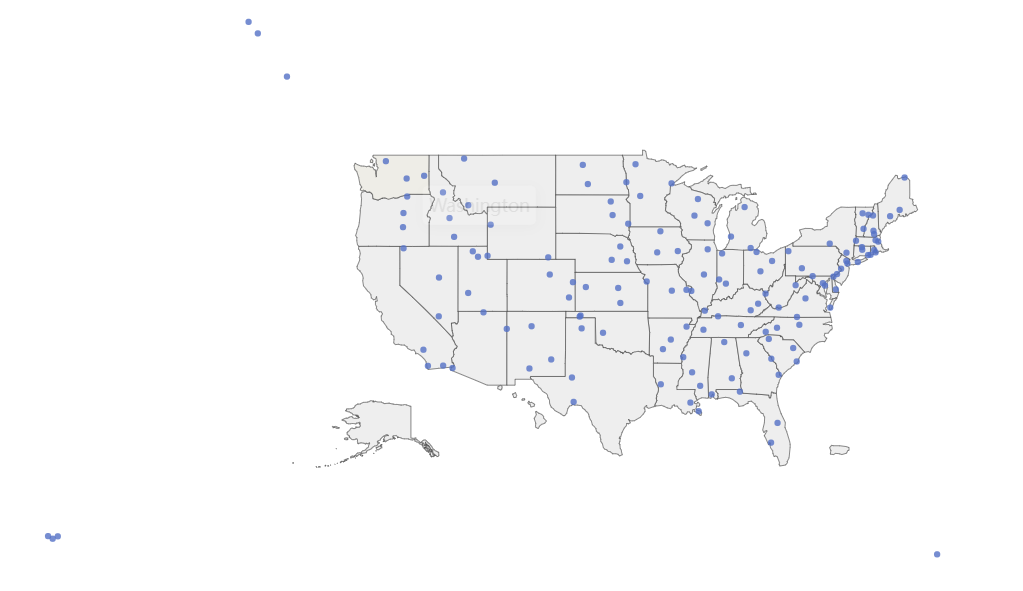
\includegraphics[width=0.9\textwidth]{map.png}

这三个地区之间距离较远,因此在考虑跨越区域的两个气象站之间的相关度时,不能将距离纳入影响因素,仅考虑其温度的相似程度。\footnote{即每天温差平方的均值}

低纬度地区有四个气象站,理论上同一地区内的气象站温度应该相近,因此我对这个地区中的气象站单独进行相关度的计算。相关度公式为$w=\frac{300}{temp}$,其中temp为气温相似度数值。
但在计算时发现有一个低纬度气象站与其他气象站温度相差很多(相差20$^\circ F$左右),此时用其他低纬度气象站温度来表征该气象站温度不甚恰当,此类气象站视为异常点。
通过观察发现,该气象站位于岛内,气温特征与美国本土相近,因此可以计算该气象站与美国本土各气象站的相关度,取最大的k个权重保留(取k=8),剩下的置为0。

高纬度地区温度与中纬度地区温度特征相差不大,并且高纬度地区数据较少,因此对于每个高纬度气象站,采用其他高纬度气象站和中纬度气象站来表征其温度,即计算它们之间的相关度。
相关度公式为$w=\frac{100}{temp}$,其中temp为气温相似度数值。取最大的k个权重保留,剩下的置为0。

中纬度地区分布的气象站比较多,各种气候均有足够多的邻域气象站,因此可以对该地区中的气象站进行单独的相关度计算。计算时考虑气象站的距离、气温相似度和纬度差。
相关度公式为$w=\frac{100}{5*(\frac{d}{R}-1)+temp+(\alpha_i-\alpha_j ) }$,其中d为距离,R为地球半径,temp为气温相似度数值,$\alpha$为气象站纬度。取最大的k个权重保留,剩下的置为0。

然后确定各气象站各天气温之间的相关度。对于不同气象站同一天的气温,其相关度等于两气象站的相关度数值;对于不同气象站不同天的气温,若相差时间为1天,则其相关度等于0.2倍两气象站的相关度数值,其余为0;
对于同一气象站不同天的气温,若相差时间为1天,则其相关度数值等于5,其余为0。采用这种先计算气象站间相关度,再计算每个点之间的相关度的方法,相比于直接计算各点之间相关度,能有效加快运算速度。

至此完成建图。

\section{结果与分析}
当预设气温异常(偏高)为$30^\circ F$,平均成功率为0.99828。

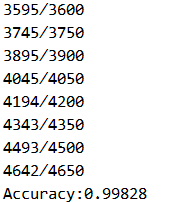
\includegraphics[width=0.2\textwidth]{accu_30.png}

当预设气温异常(偏高)为$20^\circ F$,平均成功率为0.94344。

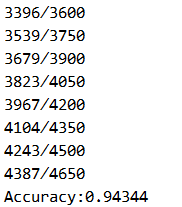
\includegraphics[width=0.2\textwidth]{accu_20.png}

当预设气温异常(偏高)为$15^\circ F$,平均成功率为0.6428。

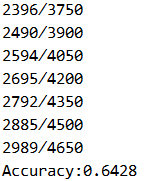
\includegraphics[width=0.2\textwidth]{accu_15.png}

将异常点输出到outlier变量中,选取其中几个点进行研究。

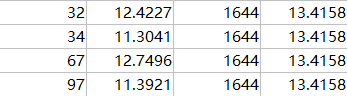
\includegraphics[width=0.3\textwidth]{outlier.png}

以上数据为气温异常为$20^\circ F$时检测失败的部分数据,其中第一列为发生异常点,第二列为该点检测出来的噪声,第三列为输出值,第四列为输出值对应检测出来的噪声。

先考虑被误判的点(以34为例),其对应第2个气象站第3天的测量气温,如下:

\begin{tabular}{|c|c|c|c|c|}
    \hline
    12 & 28 & \bfseries{18} & 36 & 27 \\
    \hline
\end{tabular}

第3天的气温$18^\circ F$比前后一天都低$10+^\circ F$,因此加上$20^\circ F$的异常值也不容易被检测出来。

其他被误判的点也有这个特点(多处于谷值),因此可以总结发生误判的点大多气温规律性较差,其附近波动较大,算法有待改进。

除此之外,我们发现基本检测失败的各点都误测为1644。

第1644个点对应第54个气象站第1天的测量气温,如下:

\begin{tabular}{|c|c|c|c|c|}
    \hline
    \bfseries{55} & 57 & 51 & 45 & 39 \\
    \hline
\end{tabular}

看起来温度分布比较正常,需要进行进一步探究。

在检验过程中,当发生误判时,令程序输出发生误判的编号与noise大于其对应噪声的索引,便于将尽可能多的误判的情况排除掉。

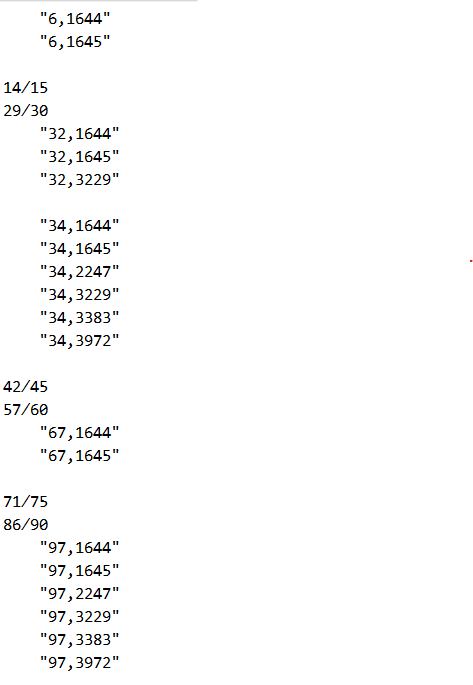
\includegraphics[width=0.4\textwidth]{error.png}

为了方便进一步了解第1644点的特征,我编写了test.m,输出与第1644点相关的各点及其权重。输出结果如下:

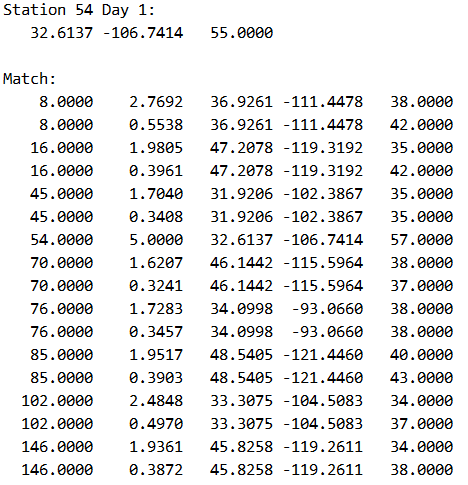
\includegraphics[width=0.4\textwidth]{1644.png}

输出结果中,第一列为气象站编号,第二列为相关度,第三、四列为气象站经纬度,最后一列为对应点的气温。
可以观察到,与1644点相关的点中除了其相邻点外,其他的气温都与第1644点气温$55^\circ F$相差很多,所以经过加权求和后必定与
实际温度相差过大。分析这样的原因,是因为计算相关度时,计算的是31天的平均的气温差,可能这里权重大只意味着整体气温规律与54号气象站的气温规律相似,
而在局部不甚相似。

由此可以提出新的改进方法:\textbf{计算温度相关性时只考虑这个点周围几天的平均气温差,而不是全部31天的平均气温差}。不过采用这种方法就无法先计算气象站之间的相关度,
只能直接计算各点之间的相关度,这样必定会增加计算的复杂度。

除了这种可能发生误判的情况,另一种情况的代表性点为3229点。

第3229个点对应第105个气象站第5天的测量气温,如下:

\begin{tabular}{|c|c|c|c|c|}
    \hline
    73 & \bfseries{70} & 47 & 48 & 54 \\
    \hline
\end{tabular}

第5天的气温$70^\circ F$比后两天高$20+^\circ F$,气温突变看起来像是发生了异常,容易发生误判,针对此类点则不容易优化方法。

\section{文件清单}
\begin{itemize}
    \item compute\_d.m: 计算两气象站之间距离
    \item compute\_temp.m: 计算两气象站之间温度相关性
    \item construct\_graph.m: 建图函数
    \item test.m: 调试使用函数
    \item detection.m: 检测异常(Main)
    \item map.py: 用于生成气象站标点地图的脚本
\end{itemize}




\bibliography{ref}


\end{document}